\chapter{Конструкторская часть}
В данном разделе будут приведены схемы алгоритмов умножения матриц, а также оценены трудоемкости каждого из алгоритмов.

\section{Представление алгоритмов}

На вход алгоритмов подаются две матрицы: $M_{1}$ размера $M \times N$, $M_{2}$ размера $N \times K$, где $M, N, K$ --- неотрицательные целые числа; на выходе - матрица $M_{3}$ размера $M \times K$.

На рисунках \ref{fig:classic} --- \ref{fig:vinograd_opt} приведены схемы трех алгоритмов умножения матриц: классического, Винограда, оптимизированного Винограда.

\clearpage

\begin{figure}[h]
	\centering
	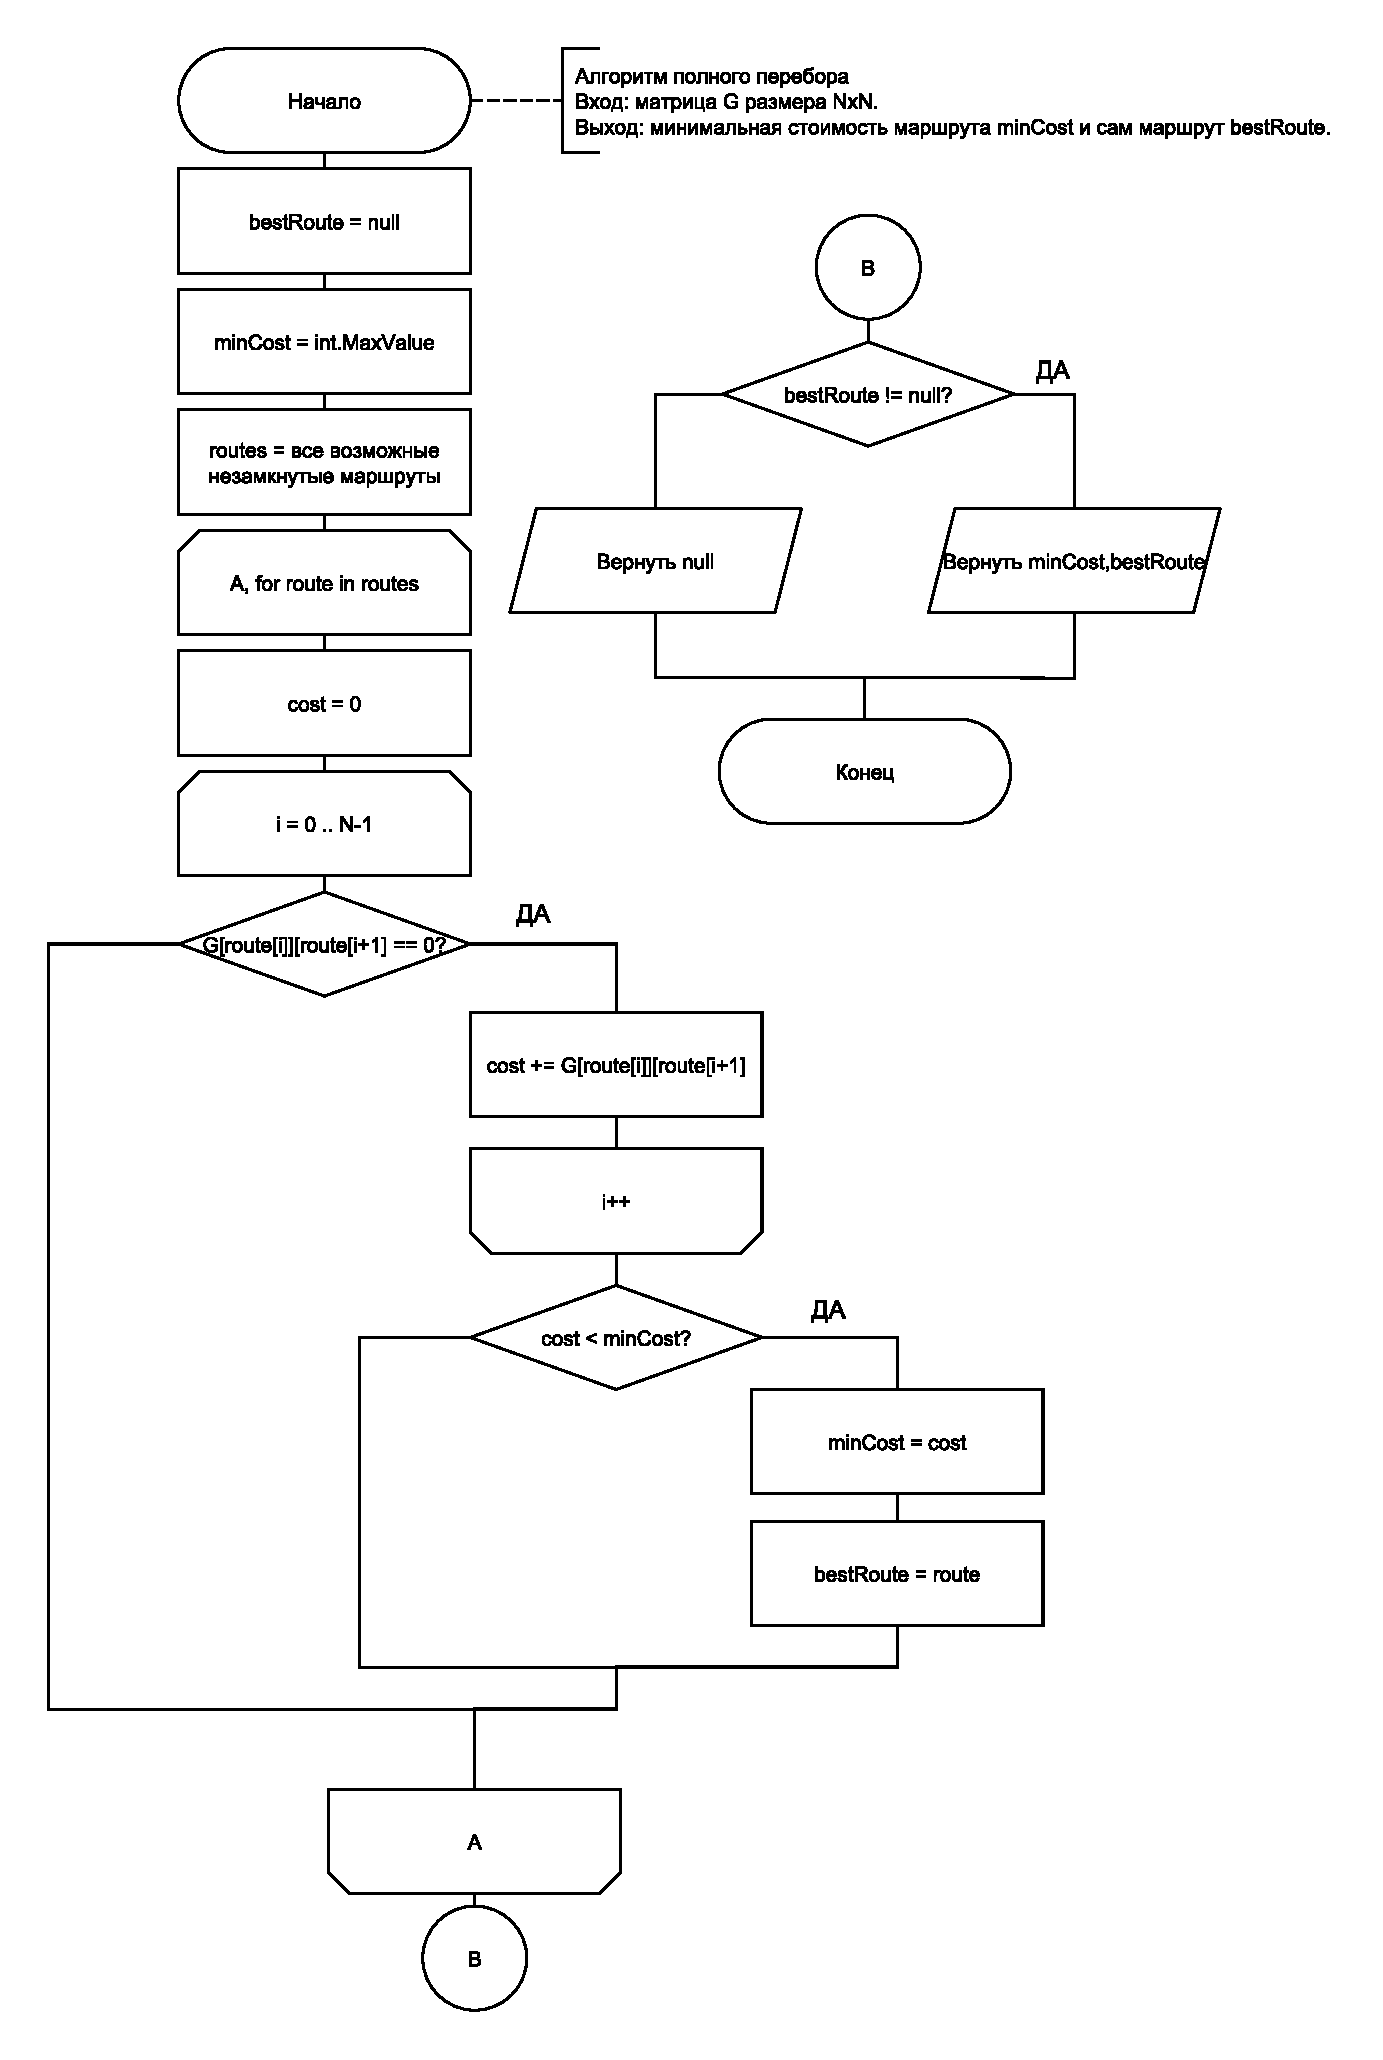
\includegraphics[scale=0.8]{img/classic.eps}
	\caption{Схема классического алгоритма умножения матриц}
	\label{fig:classic}
\end{figure}

\clearpage

\begin{figure}[h]
	\centering
	\includegraphics[scale=1]{img/vinograd-1.eps}
	\label{fig:vinograd-1}
\end{figure}
\begin{figure}[h]
	\centering
    \includegraphics[scale=0.9]{img/vinograd-2.eps}
	\caption{Схема алгоритма Винограда умножения матриц}
	\label{fig:vinograd}
\end{figure}

\clearpage

\begin{figure}[h]
	\centering
	\includegraphics[scale=1]{img/vinograd-1-opt.eps}
	\label{fig:vinograd_opt-1}
\end{figure}
\begin{figure}[h]
	\centering
	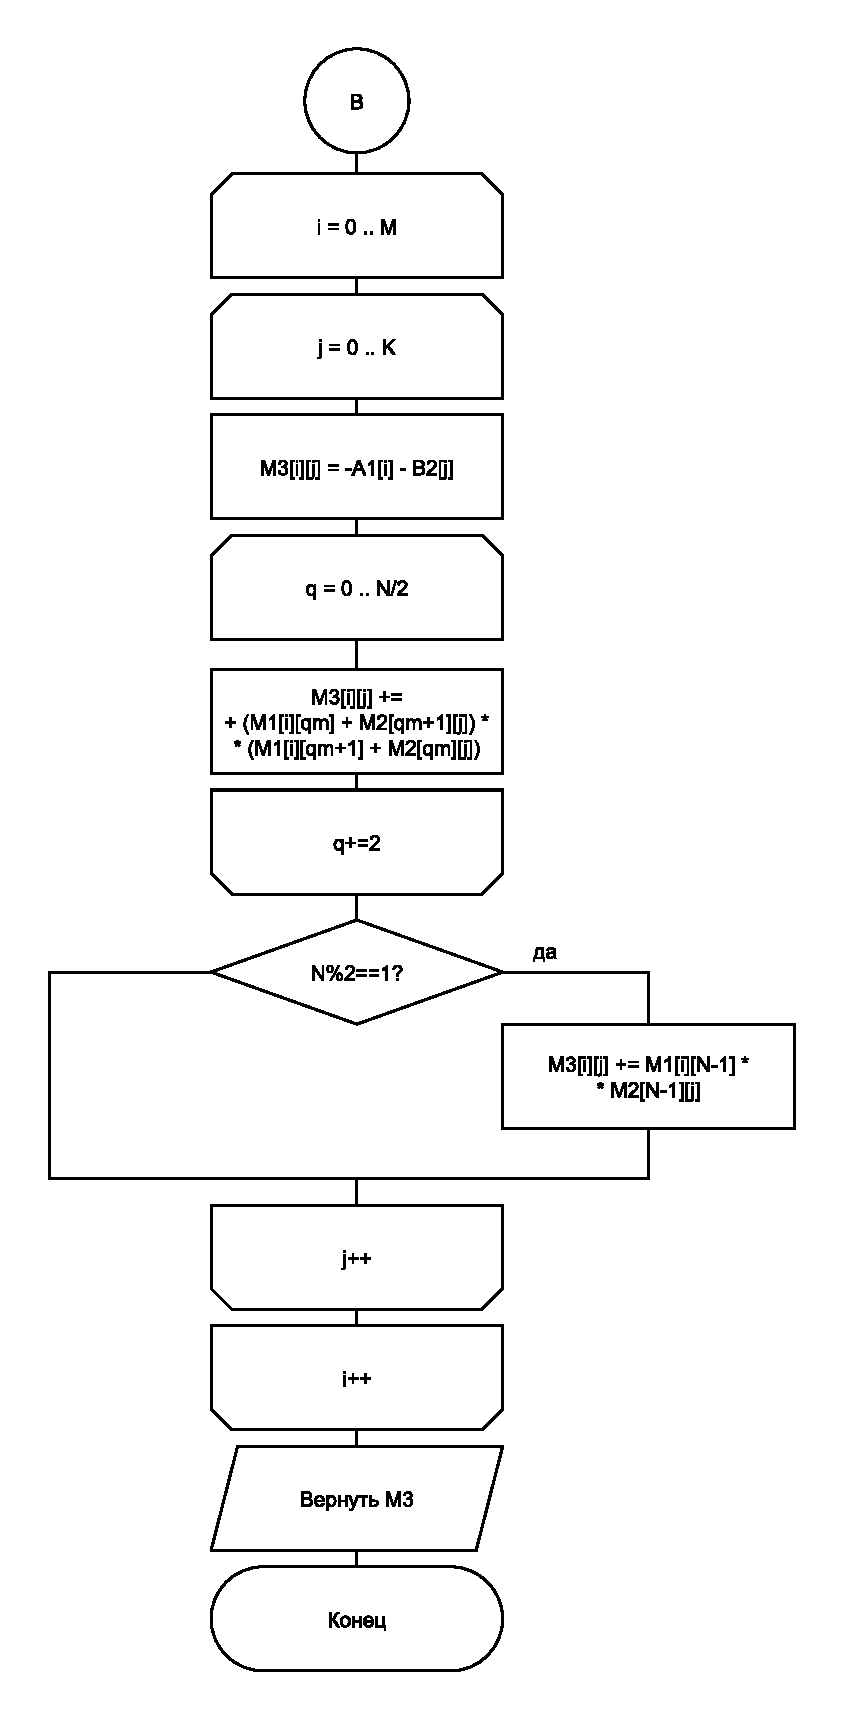
\includegraphics[scale=0.75]{img/vinograd-2-opt.eps}
	\caption{Схема оптимизированного алгоритма Винограда}
	\label{fig:vinograd_opt}
\end{figure}

\clearpage

Оптимизация алгоритма Винограда заключается:
\begin{itemize}
	\item[---] в инкременте наиболее вложенного счетчика цикла на 2;
	\item[---] в замене операций x = x + k на x += k;
	\item[---] в объединении \rom{3} и \rom{4} части алгоритма .
\end{itemize}

\section{Модель вычислений}
Для последующего вычисления трудоемкости была введена модель вычислений:
\begin{enumerate}
	\item операции из списка (\ref{for:opers}) имеют трудоемкость 1;
	\begin{equation}
		\label{for:opers}
		+, -, *, /, \%, ==, !=, <, >, <=, >=, [], ++, {-}-
	\end{equation}
	\item трудоемкость условного оператора \code{if условие then A else B} рассчитывается как (\ref{for:if});
	\begin{equation}
		\label{for:if}
		f_{if} = f_{\text{условия}} +
		\begin{cases}
			f_A, & \text{если условие выполняется,}\\
			f_B, & \text{иначе.}
		\end{cases}
	\end{equation}
	\item трудоемкость цикла рассчитывается как (\ref{for:for});
	\begin{equation}
		\label{for:for}
		f_{for} = f_{\text{инициализации}} + f_{\text{сравнения}} + N(f_{\text{тела}} + f_{\text{инкремента}} + f_{\text{сравнения}})
	\end{equation}
	\item трудоемкость вызова функции/возврата результата равна 0.
\end{enumerate}


\section{Трудоемкость алгоритмов}
В следующих частях будут рассчитаны трудоемкости представленных ранее классического алгоритма, алгоритма Винограда, оптимизированного алгоритма Винограда.
Трудоемкость инициализации результирующей матрицы учитываться не будет, поскольку данное действие есть во всех алгоритмах и не является самым трудоемким.

Введем обозначения:
\begin{itemize}
	\item[---] M --- кол-во строк первой матрицы;
	\item[---] N --- кол-во столбцов первой матрицы и кол-во строк второй матрицы;
	\item[---] K --- кол-во столбцов второй матрицы.
\end{itemize}

\subsection{Классический алгоритм перемножения матриц}

Трудоемкость стандартного алгоритма умножения матриц состоит из:

\begin{itemize}
	\item[---] внешнего цикла по $i \in [1..M]$, трудоемкость которого: $f = 2 + M \cdot (2 + f_{body})$;
	\item[---] цикла по $j \in [1..K]$, трудоемкость которого: $f = 2 + K \cdot (2 + f_{body})$;
	\item[---] цикла по $q \in [1..N]$, трудоемкость которого: $f = 2 + 10 \cdot N$.
\end{itemize}

Трудоемкость классического алгоритма равна трудоемкости внешнего цикла.
Ее можно вычислить, подставив циклы тела (\ref{for:classic}):
\begin{equation}
	\label{for:classic}
	f_{classic} = 2 + M \cdot (4 + K \cdot (4 + 10N)) = 2 + 4M + 4MK + 10MNK \approx 10MNK
\end{equation}

\subsection{Алгоритм Винограда}

Трудоемкость алгоритма Винограда состоит из:
\begin{itemize}
	\item[---] создания и инициализации массивов A1 и B1, трудоемкость которого (\ref{for:init}):
	\begin{equation}
		\label{for:init}
		f_{init} = M + K;
	\end{equation}
	
	\item[---] заполнения массива A1, трудоемкость которого (\ref{for:A1}):
	\begin{equation}
		\label{for:A1}
		f_{A1} = 2 + M \cdot (4 + \frac{N}{2} \cdot 15);
	\end{equation}
	
	\item[---] заполнения массива B1, трудоемкость которого (\ref{for:B1}):
	\begin{equation}
		\label{for:B1}
		f_{B1} = 2 + K \cdot (4 + \frac{N}{2} \cdot 15);
	\end{equation}
	
	\item[---] цикла заполнения для четных размеров, трудоемкость которого (\ref{for:cycle}):
	\begin{equation}
		\label{for:cycle}
		f_{cycle} = 2 + M \cdot (2 + K \cdot (2 + 7 + 4 + \frac{N}{2} \cdot (4 + 20)));		
	\end{equation}
	
	\item[---] цикла, для дополнения результирующего массива суммой последних нечетных строки и столбца, если общий размер нечетный, трудоемкость которого (\ref{for:last}):
	\begin{equation}
		\label{for:last}
		f_{last} = \begin{cases}
			2, & \text{размер четный,}\\
			2 + M \cdot (2 + 14K), & \text{иначе.}
		\end{cases}
	\end{equation}
\end{itemize}

Итого, результирующая трудоемкость алгоритма Винограда равна (\ref{for:final})
\begin{equation}
	\label{for:final}
	f_{final} = f_{init} + f_{A1} + f_{B1} + f_{cycle} + f_{last} \approx 12MNK
\end{equation}

Алгоритм Винограда (неоптимизированный) имеет большую трудоемкость, чем классический алгоритм.

\subsection{Оптимизированный алгоритм Винограда}
Трудоемкость оптимизированного алгоритма Винограда состоит из:
\begin{itemize}
	\item[---] создания и инициализации массивов A1 и B1 а также доп. переменной, хранящей N/2, трудоемкость которого (\ref{for:init}):
	\begin{equation}
		\label{for:init}
		f_{init} = M + K + 3;
	\end{equation}
	
	\item[---] заполнения массива A1, трудоемкость которого (\ref{for:A1}):
	\begin{equation}
		\label{for:A1}
		f_{A1} = 2 + M \cdot (4 + \frac{N}{2} \cdot 11);
	\end{equation}
	
	\item[---] заполнения массива B1, трудоемкость которого (\ref{for:B1}):
	\begin{equation}
		\label{for:B1}
		f_{B1} = 2 + K \cdot (4 + \frac{N}{2} \cdot 11);
	\end{equation}
	
	\item[---] цикла заполнения для четных размеров, трудоемкость которого (\ref{for:cycle}):
	\begin{equation}
		\label{for:cycle}
		f_{cycle} = 2 + M \cdot (2 + K \cdot (2 + 7 + 2 + \frac{N}{2} \cdot (17)) + f_{last});		
	\end{equation}
	где $f_{last}$ --- \rom{4} часть алгоритма, трудоемкость которой равна (\ref{for:last}):
	\begin{equation}
		\label{for:last}
		f_{last} = \begin{cases}
			2, & \text{размер четный,}\\
			2 + 11, & \text{иначе.}
		\end{cases}
	\end{equation}
\end{itemize}

Итого, результирующая трудоемкость оптимизированного алгоритма Винограда равна (\ref{for:final})
\begin{equation}
	\label{for:final}
	f_{final} = f_{init} + f_{A1} + f_{B1} + f_{cycle} + f_{last} \approx 8.5MNK
\end{equation}

Оптимизированный алгоритм Винограда имеет меньшую трудоемкость, по сравнению с классическим алгоритмом.

\vspace{5mm}

\textbf{ВЫВОД}

 В данном разделе были представлены схемы алгоритмов умножения матриц, а также приведены трудоемкости каждого из трех алгоритмов.

\clearpage